% Options for packages loaded elsewhere
\PassOptionsToPackage{unicode}{hyperref}
\PassOptionsToPackage{hyphens}{url}
\PassOptionsToPackage{dvipsnames,svgnames,x11names}{xcolor}
%
\documentclass[
  letterpaper,
]{krantz}

\usepackage{amsmath,amssymb}
\usepackage{iftex}
\ifPDFTeX
  \usepackage[T1]{fontenc}
  \usepackage[utf8]{inputenc}
  \usepackage{textcomp} % provide euro and other symbols
\else % if luatex or xetex
  \usepackage{unicode-math}
  \defaultfontfeatures{Scale=MatchLowercase}
  \defaultfontfeatures[\rmfamily]{Ligatures=TeX,Scale=1}
\fi
\usepackage{lmodern}
\ifPDFTeX\else  
    % xetex/luatex font selection
\fi
% Use upquote if available, for straight quotes in verbatim environments
\IfFileExists{upquote.sty}{\usepackage{upquote}}{}
\IfFileExists{microtype.sty}{% use microtype if available
  \usepackage[]{microtype}
  \UseMicrotypeSet[protrusion]{basicmath} % disable protrusion for tt fonts
}{}
\makeatletter
\@ifundefined{KOMAClassName}{% if non-KOMA class
  \IfFileExists{parskip.sty}{%
    \usepackage{parskip}
  }{% else
    \setlength{\parindent}{0pt}
    \setlength{\parskip}{6pt plus 2pt minus 1pt}}
}{% if KOMA class
  \KOMAoptions{parskip=half}}
\makeatother
\usepackage{xcolor}
\setlength{\emergencystretch}{3em} % prevent overfull lines
\setcounter{secnumdepth}{5}
% Make \paragraph and \subparagraph free-standing
\ifx\paragraph\undefined\else
  \let\oldparagraph\paragraph
  \renewcommand{\paragraph}[1]{\oldparagraph{#1}\mbox{}}
\fi
\ifx\subparagraph\undefined\else
  \let\oldsubparagraph\subparagraph
  \renewcommand{\subparagraph}[1]{\oldsubparagraph{#1}\mbox{}}
\fi


\providecommand{\tightlist}{%
  \setlength{\itemsep}{0pt}\setlength{\parskip}{0pt}}\usepackage{longtable,booktabs,array}
\usepackage{calc} % for calculating minipage widths
% Correct order of tables after \paragraph or \subparagraph
\usepackage{etoolbox}
\makeatletter
\patchcmd\longtable{\par}{\if@noskipsec\mbox{}\fi\par}{}{}
\makeatother
% Allow footnotes in longtable head/foot
\IfFileExists{footnotehyper.sty}{\usepackage{footnotehyper}}{\usepackage{footnote}}
\makesavenoteenv{longtable}
\usepackage{graphicx}
\makeatletter
\def\maxwidth{\ifdim\Gin@nat@width>\linewidth\linewidth\else\Gin@nat@width\fi}
\def\maxheight{\ifdim\Gin@nat@height>\textheight\textheight\else\Gin@nat@height\fi}
\makeatother
% Scale images if necessary, so that they will not overflow the page
% margins by default, and it is still possible to overwrite the defaults
% using explicit options in \includegraphics[width, height, ...]{}
\setkeys{Gin}{width=\maxwidth,height=\maxheight,keepaspectratio}
% Set default figure placement to htbp
\makeatletter
\def\fps@figure{htbp}
\makeatother

\makeatletter
\makeatother
\makeatletter
\@ifpackageloaded{bookmark}{}{\usepackage{bookmark}}
\makeatother
\makeatletter
\@ifpackageloaded{caption}{}{\usepackage{caption}}
\AtBeginDocument{%
\ifdefined\contentsname
  \renewcommand*\contentsname{Table of contents}
\else
  \newcommand\contentsname{Table of contents}
\fi
\ifdefined\listfigurename
  \renewcommand*\listfigurename{List of Figures}
\else
  \newcommand\listfigurename{List of Figures}
\fi
\ifdefined\listtablename
  \renewcommand*\listtablename{List of Tables}
\else
  \newcommand\listtablename{List of Tables}
\fi
\ifdefined\figurename
  \renewcommand*\figurename{Figure}
\else
  \newcommand\figurename{Figure}
\fi
\ifdefined\tablename
  \renewcommand*\tablename{Table}
\else
  \newcommand\tablename{Table}
\fi
}
\@ifpackageloaded{float}{}{\usepackage{float}}
\floatstyle{ruled}
\@ifundefined{c@chapter}{\newfloat{codelisting}{h}{lop}}{\newfloat{codelisting}{h}{lop}[chapter]}
\floatname{codelisting}{Listing}
\newcommand*\listoflistings{\listof{codelisting}{List of Listings}}
\makeatother
\makeatletter
\@ifpackageloaded{caption}{}{\usepackage{caption}}
\@ifpackageloaded{subcaption}{}{\usepackage{subcaption}}
\makeatother
\makeatletter
\@ifpackageloaded{tcolorbox}{}{\usepackage[skins,breakable]{tcolorbox}}
\makeatother
\makeatletter
\@ifundefined{shadecolor}{\definecolor{shadecolor}{rgb}{.97, .97, .97}}
\makeatother
\makeatletter
\makeatother
\makeatletter
\makeatother
\ifLuaTeX
  \usepackage{selnolig}  % disable illegal ligatures
\fi
\IfFileExists{bookmark.sty}{\usepackage{bookmark}}{\usepackage{hyperref}}
\IfFileExists{xurl.sty}{\usepackage{xurl}}{} % add URL line breaks if available
\urlstyle{same} % disable monospaced font for URLs
\hypersetup{
  pdftitle={Los Faros Etéreos},
  pdfauthor={Diego Figueiras},
  colorlinks=true,
  linkcolor={blue},
  filecolor={Maroon},
  citecolor={Blue},
  urlcolor={Blue},
  pdfcreator={LaTeX via pandoc}}

\title{Los Faros Etéreos}
\author{Diego Figueiras}
\date{2024-01-22}

\begin{document}
\maketitle
\ifdefined\Shaded\renewenvironment{Shaded}{\begin{tcolorbox}[borderline west={3pt}{0pt}{shadecolor}, sharp corners, interior hidden, breakable, boxrule=0pt, enhanced, frame hidden]}{\end{tcolorbox}}\fi

\renewcommand*\contentsname{Table of contents}
{
\hypersetup{linkcolor=}
\setcounter{tocdepth}{2}
\tableofcontents
}
\bookmarksetup{startatroot}

\hypertarget{portada}{%
\chapter*{Portada}\label{portada}}
\addcontentsline{toc}{chapter}{Portada}

\markboth{Portada}{Portada}

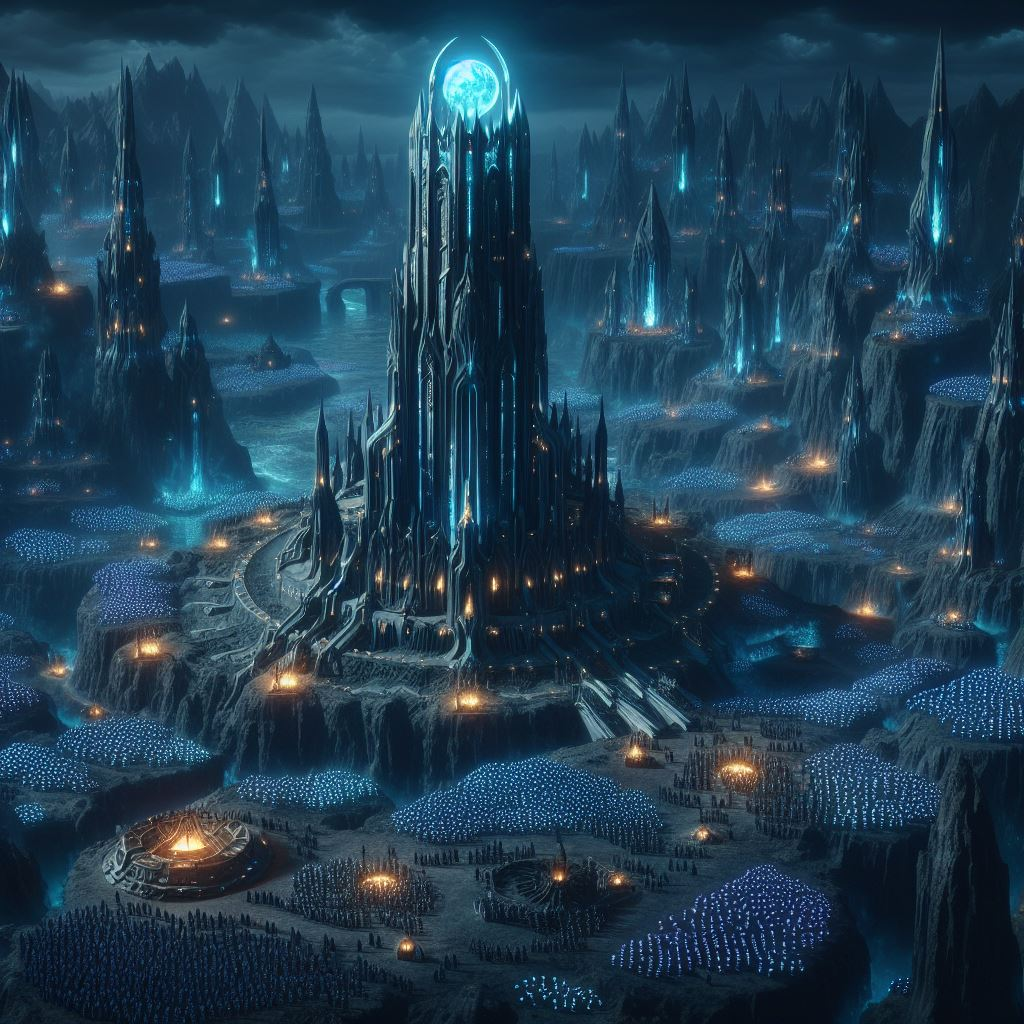
\includegraphics{portada.jpg}

\bookmarksetup{startatroot}

\hypertarget{capuxedtulo-1-la-diosa}{%
\chapter{Capítulo 1: La Diosa}\label{capuxedtulo-1-la-diosa}}

\bookmarksetup{startatroot}

\hypertarget{capuxedtulo-2-el-princeso}{%
\chapter{Capítulo 2: El Princeso}\label{capuxedtulo-2-el-princeso}}

La victoria había sido fácil, demasiado fácil, lo cual solía poner a
Gaspar Lobera, el Príncipe Zafiro, como lo llamaba la plebe, de mal
humor. Nada más empezar el duelo habían bastado las cinco runas Sped en
las placas de acero que cubrían sus botas para propulsarlo a gran
velocidad y salvar la distancia entre él y el arzobispo de Conztanza. Al
igual que el hermano de Gaspar, el arzobispo no era ningún caballero
rúnico, sino más bien un mago. Peligroso si le daba tiempo para conjurar
sus hechizos, pero vulnerable a corta distancia. Ni siquiera tenía la
espada alzada, sino que pasaba las páginas de su grimorio que flotaba a
un costado. Lo primero que el duque hizo fue cortar el libro en dos de
un tajo de Tizón, la espada ancestral de la familia Lobera, cuyas runas
incandescentes emitían el brillo zafiro que daba lugar al apodo de su
portador.\\
El arzobispo activó las runas en su guantelete, pero antes de que
pudiera terminar de leerlas, el duque ya estaba contrarrestando su
hechizo Faëran conjurando Angaz en tres menor, desviando el haz de luz
dorado. Se fue a estallar contra la custodia mágica que protegía a los
espectadores. La explosión hizo que el estadio retumbara en gritos de
jolgorio. Al mismo tiempo, Tizón arremetía contra su rival. La
translúcida custodia mágica del arzobispo contuvo la ira de la espada, y
su propia arma por fin se alzó para unirse a la contienda. Pero para
cuando la primera runa grabada en el filo se prendió en un verde
esmeralda que indicaba su naturaleza Püsle, el duelo ya había terminado.
Tres rápidas estocadas de Tizón y la fina custodia turquesa que lo
envolvía se vino abajo, disipándose en un millar de motas cristalinas.\\
\strut \\
---¡El vencedor es Gaspar Lobera, Duque de Lisandra y de Irinea, Paladín
de la orden de los caballeros rúnicos, Comandante de las Fuerzas de la
Liga, e hijo del Hechicero Supremo de la Liga de Magos!\\
Tras los aplausos, las irritantes ovaciones y todas las ceremonias, el
duque se acercó al arzobispo y le puso una mano en el hombro.\\
---Lo siento por el grimorio ---le dijo. Este yacía en el suelo
fragmentado en dos, abrasado en su mayor parte---. Mándale un recibo a
mi Maestro de Armas y te reembolsaré cualquier valor que pidas.\\
---No pasa nada ---respondió el elfo ---. Tengo centenares como este.
Buena pelea, ojalá hubiera estado a la altura.\\
---No te voy a mentir, pudiste haber luchado mejor. Espero poder
enfrentarme a tu primo en el torneo de Eleonora, que ya va a ser pronto
---dijo, quitándose el yelmo. Tenía cabello y barbas negros, ojos
azules, tez grisácea y nariz aguileña.\\
---Lo pondré sobre aviso, pues, para que se vaya preparando.\\
\strut \\
Ambos montaron sobre sus respectivos pegasos, saludaron a los setenta
mil espectadores, y abandonaron el estadio a través de uno de los
múltiples arcos que adornaban la cima de la cúpula del coliseo. Cuando
el duque llegó a los establos de la basílica de Diamanthora, y una vez
sus escuderos lo alcanzaron y lo ayudaron a quitarse el arnés y
desmontar de Gabriela, y también a quitarse la armadura adornada con
zafiros, se dirigió a reunirse con su padre.\\
Lo había dejado cuidando de su pequeña hija, Sofía, en sus aposentos de
lujo. Tenían una reunión familiar en breves, así que se dio prisa a
través del laberinto de escaleras de mármol y de funcionarios del
imperio. Tocó en la puerta, pasó la llave y entró sin pedir permiso. Los
encontró tumbados sobre el suelo y sonrió. Padre la había vuelto a
convencer para jugar a hacerse los muertos y así poder tomarse una
siesta sin ser molestado.\\
\strut \\
---Sofía, ya puedes dejarte de juegos, que ya has ganado. El abuelo está
durmiendo.\\
La niña de pelo rizado y ojos esmeralda, a la cual no se le daba muy
bien jugar a los muertos ya que no era capaz de contener su entusiasmo
ni estando inmóvil en el suelo, se levantó con rapidez y, patosamente,
dio unos pasos para confirmar lo dicho por su padre.\\
---¡No vale, abuelo!\\
Le agitó el hombro con sus regordetas manos, pero el anciano elfo ni se
inmutó. Viéndolo ahí, con su larga barba blanca a juego con su
cabellera, piel del color de la ceniza bajo la luz de la luna, nariz
bulbosa y rosada, vestido con una bata y zapatilla de andar por casa, y
roncando levemente, no pudo evitar sonreír. Costaba creer que estuviera
ante una de las personas más ricas y poderosas del mundo.\\
---¡Padre, despierte! ¡Padre!\\
El anciano abrió un poco los ojos. Miró de un lado a otro, bostezando y
confuso.\\
---¿Dónde estoy? ¿Dónde está Emma? Hablad con Emma, ella os lo
solucionará ---dijo, volviéndose hacia un lado y durmiéndose una vez
más.\\
---Emma ha muerto hace años, y estás en la basílica de Diamanthora, a
dos días de los votos. ¡Padre! ¡Despierte! ¿Se ha tomado la medicina?\\
---¡Abuelo!\\
La niña lo volvió a agitar por el hombro, y este aprovechó para
agarrarla y provocarle cosquillas.\\
---¡Ya va, ya va! ---dijo, mientras la pequeña reía.\\
Al duque ni siquiera le hacía falta una respuesta, se acercó al baúl de
viaje y sacó una caja de madera repleta de pócimas. Padre siempre se
olvidaba de la medicina, y aunque se acordase, no sabía cuál era la
dosis correcta. Gaspar era el que estaba al cargo de sus cuidados.\\
---Tenemos la reunión esa que concertaste esta mañana, ¿recuerda?
---dijo entretanto ponía la botellita de cristal a la luz del sol y la
golpeaba con el dedo, examinando la disolución.\\
El anciano se levantó trabajosamente mientras ponía a la niña a un
lado.\\
---¿Reunión?\\
---Sí, con toda la familia y\ldots{} ya sabes. Lo de\ldots{}\\
---Ah, sí ---Lo fulminó con la mirada, un ojo verde esmeralda como el de
Sofía, y el otro nublado por cataratas---. Todo eso.\\
Abrió la boca para que Gaspar le diera la cucharada de medicina y tragó,
arrugando el rostro con desagrado.\\
---Bueno, pues no perdamos más tiempo. ¿Dónde están Colatho y mi
sombrero?\\
---¡Aquí! ---respondió Sofia, trayendo el lujoso bastón con grabados
rúnicos y adornos de diamantes en su extremo, y también el sombrero
picudo de la Universidad de Dacaroth.\\
---Primero dejemos a Sofía con su madre. Carmela no necesita asistir, ¿o
sí? --- indagó el duque.\\
Padre negó con la cabeza mientras tomaba las posesiones que la niña le
ofrecía. El bastón era tan largo que la pequeña apenas podía sostenerlo
por mucho tiempo. La agarró a ella también en sus brazos y la puso sobre
sus hombros.\\
---Muy bien, en ese caso vayamos ---dijo Gaspar.\\
---Tu padre es todo negocios, nada de diversión ---le dijo padre a la
niña, la cual le quitó su sombrero de mago y se lo puso ella misma en la
cabeza. Le quedaba tan grande que le ocultaba los ojos.\\
---Papá es un hombre muy importante, todo el mundo lo dice.\\
---Sin lugar a dudas ---respondió el anciano, sonriéndole a Gaspar.\\
---¿Tú también eres importante, abuelo?\\
---Nah. Yo solo soy un viejo idiota. Un viejo que ni ve ratas.\\
---¿Es por culpa de tu ojo ciego?\\
---Sí, tal vez. Pero por suerte el que está sano lo ve todo.\\
\strut \\
Bajaron a la octava planta del ala oeste de la basílica. La habían
reservado entera para que toda la familia pudiera hospedarse durante las
elecciones, bajo el pretexto de que padre, en sus funciones como
Hechicero Supremo, tuviera acceso rápido a posibles consultas de última
hora. Dejaron a la niña en las habitaciones de Gaspar y su esposa, la
cual le dio un beso en la mejilla antes de despedirse, y luego volvieron
a subir por las escaleras de mármol, rumbo al comedor privado de la
duodécima planta. Allí era donde iba a tener lugar la reunión.\\
---Ya sabes que no me gusta que te quedes dormido mientras estás
echándole un ojo a Sofía ---dijo el duque mientras caminaban.\\
Padre sacudió la mano, como descartando el comentario.\\
---Le puse siete custodias encima. Ni aunque la metieras en un barril de
ácido y la tirases en una catapulta le pasaría nada. Y cerré la puerta
con llave.\\
Padre aceleró el paso una vez llegaron al corredor que conducía a las
estancias, sujetando a Colatho por el centro y musitando algo que Gaspar
no pudo entender pero que no auguraba nada bueno. Se sacó el
Loberonicón, su grimorio personal, de un bolsillo interior de su bata y
este se abrió solo, quedándose flotando a un lado. Las páginas pasaron
como si una ventisca las estuviera hojeando, y se detuvieron en un
pasaje de glifos que brillaron en una multitud de colores cuando padre
los leyó rápidamente. Las inmensas puertas de roble vigiladas por
guardias se abrieron como si un ariete las hubiera golpeado, y pudieron
ver que ya había gente dentro.\\
Gaspar discernió a su hermana Aurora, sentada a lado de la cabecera de
la mesa. Era una elfa de cabello plateado, piel gris, y ojos azules
marcados por ojeras rosadas. Ostentaba varios títulos, pero el más
importante de todos era el de senescal de padre. Donde Gaspar era el
comandante de las fuerzas militares de la familia, Aurora era la que
llevaba la mayoría de los asuntos administrativos y legales, y actuaba
como portavoz de padre en cualquier circunstancia en donde estuviera
ausente.\\
También vio a su primo Hilario, el idiota fanfarrón, susurrándole algo a
Aurora al oído, a su hermano Gespirito sujetando una copa de vino, a la
tía Isolina, la Reina de las Arañas, a lado de la chimenea, al tío
Fermín, que en realidad no era tío de nadie pero lo llamaban así,
picoteando un poco de queso, y a su hermana Leopolda riéndose de algo
que el primo Gustavo estaba diciendo. Twylwarlais II, el emperador,
también estaba allí, a solas en un extremo de la mesa. Todos se
asustaron cuando las puertas golpearon las paredes con una fuerza tal
que parecía que las bisagras fueran a estallar.\\
---Hey, papá ---dijo Gespirito, acercándose. Cuando entraron, Gaspar se
dio cuenta de que había más gente en la sala de la que esperaba. El tío
Filisindro, que era tío de verdad, y varios sirvientes ---. He publicado
mi nueva crítica de teatro en el Relaciones. A ver qué te parece esto:
---Desenrolló el periódico---. "Aunque me siento compungido a la par que
anonadado por el coraje, acaso incluso atrevimiento de la decisión tan
exacerba y oh siempre tan adamantina del aclamado director y dramaturgo
Eodär Illiden por incluir a un actor humano desempeñando el papel del
hidalgo alto elfo\ldots"\\
---Gespirito, chúpame la polla, anda ---le espetó padre. Colgó su
sombrero de la percha más cercana y dejó a Colatho en una esquina. Luego
se volvió al resto, fulminándolos con su ojo esmeralda ---. Quiero saber
quién de vosotros fue el retrasado mental que le dijo al rey de
Jalolandria que estamos interesados en comprar tierras.\\
Los que estaban sentados se apresuraron a levantarse, y los que ya
estaban de pie empezaron a revolotear de un lado a otro. Gespirito dio
un largo trago de su copa, con los ojos muy abiertos. Los guardias que
estaban afuera, en el corredor, cerraron las puertas, y los sirvientes
se apresuraron a llenar las copas que estuvieran vacías.\\
---Uhmmm\ldots{} padre, creo que\ldots{} ---empezó Gaspar.\\
---No te he hablado a ti, princeso ---lo interrumpió padre ---. Le hablo
a esta jauría de villanos y sicofantes a la que llamo familia.\\
Dio largos y angustiados pasos hacia la cabecera de la larga mesa
mientras el Loberonicón lo seguía, levitando. Aurora se volvió a
sentar.\\
---Papá, yo no\ldots{} yo\ldots{} no sé quién, pero yo\ldots{}\\
---Sí, sí, tú no has sido, Aurora, eso ya lo sé. Ni capaz serías de algo
tan astuto tampoco. Ponte tranquila, que te va a dar una taquicardia,
anda.\\
Aurora parecía querer llorar, aunque esa era su cara por defecto cada
vez que padre le reñía.\\
Este tomó asiento y suspiró. Gaspar se sentó enfrente de Aurora, y el
resto procedieron a sus correspondientes lugares.\\
---¿Dónde está Valentino? ---preguntó entonces el duque, notando su
ausencia.\\
---Sí, ¿dónde está el cretino? Lo conozco desde que era corrida
tocándome los cojones desde dentro, seguramente fue él ---dijo padre.\\
---Tarde, como siempre ---respondió el tío Filisindro. No tenía a su
sobrino en muy alta estima.\\
---Padre, ¿qué es lo que ocurre? ---preguntó Leopolda, tratando de poner
la voz más angelical que era capaz.\\
Era la hermana más pequeña, y la que mejor podía apaciguar a padre,
después de Sofía, claro.\\
---Sí, padre, ¿qué ocurre? ---dijo Gespirito.\\
---"Qué ocurre", como si no lo supieras de sobra, Gespirito. No han
pasado ni dos días y ya habéis ido con el cuento a todo el mundo. Que
parece que nunca dais aprendido la lección: yo me entero de todo. ¿Qué
pasa, que ya has vuelto a comprar bonos del imperio y has querido ir de
chupa anos a hacerle dinero a tus amigos maricones?\\
---No, papá, no fui yo. Esta vez lo juro.\\
---También lo jurabas cuando financiamos la guerra entre Conztaza y
Xydalia.\\
---No recuerdo haber jurado nada durante aquel episodio, pero te repito
que lo siento. También debo decir que encuentro altamente ofensivo que
te refieras a los elfos silvestres como "maricones". Son gente bella y
apasionada que\ldots{}\\
---Cállate la boca. Abraza-árboles de mierda y defensores del tojo, con
sus gilipolleces de género fluido y arte de mierda que hasta un niño
subnormal podría hacer. Hablando de subnormales, vosotros ---Miró a los
primos Hilario y Gustavo --- ¿Le habéis ido con el cuento a mi hermano?
Dije que el tema no debía salir de entre los que estábamos en la sala en
ese momento, sin importar quién fuera.\\
---Yo no le dije nada, lo juro ---afirmó Hilario.\\
---Ni yo.\\
---A lo mejor fue tu querido primogénito. El princeso ahí sentado, todo
calladito ---sugirió Aurora, señalando a Gaspar, el cual se limitó a
alzar los brazos, confuso ---. Sí, sí, hazte el tonto. ¿Cuánto te pagan
los gremios por venderle a niños muñequitos de acción hechos a tu
semejanza?\\
---Lo de que son para niños es una sugerencia, Aurora ---señaló
Gespirito.\\
---Si Val estuviera aquí, estoy seguro de que encontraría una forma de
hacer un chiste pervertido sobre tu pregunta, Aurora ---repuso Gaspar.\\
---El princeso jamás me traicionaría y eso es todo lo que tengo que
decir al respeto ---se limitó a decir padre --- ¿Y tú qué, Isolina? ¿Vas
a decir algo con al menos una pizca más de inteligencia que Aurora u os
mando a las dos a la puta cocina a plancharme los calzoncillos?\\
La tía alzó la cabeza con orgullo.\\
---Vete a la mierda, Lisardo ---dijo---. Yo no soy como tus hijos para
que me hables así. Y no, no dije nada, tus asuntos no me incumben.\\
---No te incumben excepto cuando necesitas dinero para pagarte los
divorcios. ¡Y te hablo como me de la puta gana mientras estés bajo mi
techo!\\
---Técnicamente es techo del imperio, que estamos en la basílica
---señaló Aurora, sin darle la cara a padre.\\
---Lo dicho, mi techo, ¿o has nacido ayer? ---Padre miró al emperador
Twylwarlais II, como si recién notase su presencia ---. Sin ofender,
Firulais.\\
---No hay ofensa ninguna, señor. Y no, antes de que pregunte, no dije
nada a nadie.\\
\strut \\
El emperador era un alto elfo de la edad de Valentino, apenas treinta y
dos años. Cuando su padre murió, poco faltó para que su trono fuera
usurpado por sus generales y sus tierras confiscadas. Fue padre quien
consiguió sentenciarlos a muerte y tomar al joven emperador bajo su
tutela, criándolo como si fuera un hijo más. Consideraba a Gaspar y al
resto como hermanos.\\
En ese momento las puertas se volvieron a abrir con el mismo melodrama
de antes, lo cual solo podía significar una cosa: Valentino. Gaspar
tornó la cabeza para confirmarlo. Decían que su hermano era la viva
imagen de su padre cuando este era joven. Alto, de ojos verdes, pelo
negro azabache y largo hasta los hombros, piel gris pálido y barba bien
recortada. Su parecido con padre iba acentuado por su indumentaria. Era
el único de los hermanos en haber estudiado en Dacaroth, la universidad
de magia y runismo, y en conseguir que le concedieran el bastón y el
sombrero que oficialmente le daban el título de mago. Gaspar conocía el
lenguaje de runas necesario para usar artefactos encantados, pero
Valentino no solo conocía ese lenguaje, sino también el complejo léxico
y sintaxis de glifos necesario para producir las runas. Eso significaba
que podía conjurar hechizos sin necesidad de artefactos enrunados,
simplemente leyendo los textos de glifos, ya bien fuese en papel o desde
la memoria. A menos que fuesen enrunados, la mayoría de hechizos solían
requerir docenas y docenas de páginas de glifos para ser conjuradas, y
Valentino y padre se conocían un puñado de ellos de memoria, sin ni
siquiera necesidad de consultar sus grimorios. Eso les daba ventaja
sobre las runas en que podían alterar las propiedades de los hechizos al
tiempo que los conjuraban, en vez de estas estar fijadas, pero a costa
de que les llevaba más tiempo. Gaspar se sabía dos, ambos hechizos de
custodia mágica, pero para todo lo demás dependía de artefactos como
Tizón.\\
\strut \\
---Qué coño pasa, hijos de puta ---dijo Valentino mientras caminaba
dentro. Dejó su sombrero y abrigo de cuero en la percha, el bastón a
lado del de padre, y dio la vuelta a la mesa, dándole un fuerte abrazo a
Leopalda al pasar a su lado, haciendo como que le daba un puñetazo a
Gespirito en el mentón al pasar al lado del suyo, y estampándole un beso
a Aurora en la mejilla. Esta reaccionó como si un mosquito la hubiera
picado.\\
---Hala, insultando a nuestra querida y difunta madre ---le recriminó
Gaspar, pero a Valentino el comentario le pareció hilarante y su
respuesta fue una mera carcajada.\\
---Ya te oigo gritar desde fuera, viejo. ¿Qué pasa, que hoy toca
recordarles a tus hijos lo decepcionantes que somos, lo mucho que
tenemos que estarte agradecidos de siquiera respirar, y que somos todos
unos inútiles? ---dijo, dándole un beso a padre en la frente al pasar a
su lado y revolviéndole la melena.\\
---No, pero si lo dijera tendría toda la razón del mundo ---respondió
este, haciendo aspavientos con la mano para que se apartara y
reordenándose el pelo. ~\\
---"Y te hablo como me de la puta gana mientras estés bajo mi techo." Si
me dieran media moneda de bronce cada vez que he escuchado eso, ahora
mismo sería tres veces más rico, y eso que ya soy asquerosamente rico.
Viejo, vestido así parece que te hemos rescatado de mendigar en las
calles.\\
---Y tú vestido así pareces un niño de papá al que este le dio toda la
riqueza de la que presume ---respondió padre.\\
Valentino le dio un apretón a Gaspar en el hombro y se sentó a su
lado.\\
---¿Quién coño plancha calzoncillos en la cocina, por cierto? ---dijo
entre risas --- ¿No te decidías por un comentario machista y tuviste que
hacer dos al mismo tiempo, viejo?\\
Aurora y la tía Isolina rieron. Padre los ignoró y señaló al tío Fermín
con el dedo.\\
---Fermincito, ¿qué tienes que decir?\\
---Quizás hayan sido los Parceló los que se chivaron---sugirió el tío
Fermín, que parecía ya tener la respuesta preparada ---. Son los únicos
a los que de momento hemos contactado para empezar negociaciones.\\
---Imposible que sepan nada, solo les hemos mandado a nuestras putitas a
que los convenzan de venir a Diamanthora ---le dijo padre. "Putitas" era
como llamaba a los ministros del imperio---. Y aunque lo supieran, ¿por
qué habían de decir nada? Deben de estar como quinceañeras ante la idea
de que siquiera contactemos con ellos, no van a arruinar su oportunidad
de escapar del lodazal inmundo que son sus tierras. El lodazal que es
todo el nombre de su familia, mejor dicho.\\
---Fui yo ---dijo entonces Valentino, sin más.\\
Los tíos Fermín y Filisindro intercambiaron miradas anonadadas, y los
primos se rieron, pensando que era una broma. Pero los hermanos
palidecieron, pues como había vaticinado el anciano, ya se temían que
seguramente había sido él.\\
---Aham\ldots{} ---se limitó a decir padre, apoyando la cabeza sobre sus
manos cruzadas y con la cara inexpresiva.\\
---¿Qué estás diciendo, Valentino? ---preguntó la tía Isolina,
atónita.\\
---Estabais hablando sobre quién filtró nuestros planes de comprar
tierras, ¿no? Bueno, pues os estoy diciendo que fui yo. Misterio
resuelto, ya no nos intimides más, viejo, que el primo Gustavo ahí está
usando toda su fuerza de voluntad para evitar cagarse en los pantalones
y ya casi puedo verle la mierda salirle por la boca.\\
Gaspar miró a su primo, el cual, en efecto, estaba pálido y
tembloroso.\\
---Val, eres un idiota ---dijo Aurora.\\
---Sí, Val, ¿qué cojones? ---añadió Gespirito --- ¿Traicionando a tu
propia familia? Media estrella de cinco, no te recomiendo.\\
Hizo como que escribía en un cuaderno imaginario.\\
---Deja el drama para tus críticas pedorras de teatro, Gespirito. Estoy
acelerando nuestros planes.\\
---¿Acelerando los planes? ---dijo Twylwarlais ---. Si los altos elfos
se enteran de esto, adiós planes. No van a dejar que unos simples
dro\ldots{} que unos elfos oscuros los igualen en poder, o incluso
superen.\\
---Ya los superamos, es solo que nadie te lo ha dicho todavía. Y uh,
¿ibais a decir la palabra que empieza por D, majestad Firulais?
---respondió Valentino con una sonrisa de oreja a oreja ---. Puedes
llamarnos drows todo lo que quieras, entre nosotros lo hacemos todo el
tiempo, ¿verdad, viejo drow? Tenemos a papá drow, princeso drow, mi
hermana la drow suprema, etcétera.\\
---Val\ldots{} ---Aurora puso los ojos en blanco.\\
---No te olvides de capullo drow ---dijo Gaspar, apoyando la mano en la
espalda de Valentino.\\
---Gespirito y Leopalda son solo medio drows, pero siguen siendo
oscuros. Mala hierba nunca muere.\\
---¡Val!\\
---¿Qué?\\
---Padre ha sido muy claro sobre la privacidad de nuestros planes
---dijo Gaspar.\\
---¿Y qué? Uno no va al mercado a hacer la compra en susurros. Hay que
gritar para anunciarse.\\
---¿Por qué no nos dijiste nada primero? Ninguno de nosotros puede
actuar por su cuenta, de lo contrario esto sería un circo ---dijo la tía
Isolina.\\
---Vosotros no podéis actuar por vuestra cuenta, yo puedo hacer lo que
me de la puta gana. Estoy aquí por mutuos intereses, no solo por ser
miembro de la familia, ¿recordáis? Tengo mis propios Faros.\\
\strut \\
Cuando padre no era más que un sargento mayor miembro de la por aquel
entonces familia menor de barones Lobera, viendo la necesidad de los
caballeros rúnicos y de los magos de batalla para tener acceso inmediato
a recursos de éter, diseñó los Faros Etéreos. Por aquel entonces era un
joven mago y hechicero, graduado de Dacaroth desde hacía poco pero con
muchas ambiciones. Conjurar hechizos requería del uso de ese gas
producido naturalmente por el cuerpo conocido como éter. Cuando un
caballero rúnico o un mago consumía cierta cantidad de éter, debía
reponer fuerzas antes de reanudar el lanzamiento de hechizos, de lo
contrario la magia le carcomía la carne y los huesos, drenando toca la
energía y materia que podía sustraer del cuerpo hasta matarlo. Pero
aquello había cambiado con los Faros.\\
Torres con una gran esfera de luz en sus cimas, de ahí el nombre,
absorbían toda partícula de éter que podían extraer del área en que eran
construidos, proporcionando una fuente sostenible y continua del gas que
se podía almacenar en bolas de cristal. Cuando conjuraban sus hechizos,
los magos no necesitaban más que sostener las esferas en sus manos para
restablecer sus fuentes de éter. Muchos académicos y nobles afirmaban
que esto había sido el factor determinante para que el imperio de
Diamanthora ganase la guerra contra los Ascaroth, y desde entonces la
economía y el uso de la magia habían cambiado para siempre. Las esferas
de éter se habían convertido en una moneda más valiosa que el oro o la
plata, convirtiendo a los Lobera en los banqueros más adinerados del
mundo en cuestión de unos pocos años, y la magia ya no era una
disciplina reservada para unas pocas familias aristocráticas de elfos.
Enanos, hadas, e incluso algunos humanos podían aprender runismo y
conjurar hechizos, con variados grados de sofisticación entre ellos,
pero la oportunidad presente.\\
Desde el día en que se convirtió en mago, Valentino había empezado a
construir sus propios Faros, con sus propios diseños y adquiriendo sus
propias tierras. Padre lo consideraba un simple ladrón y aprovechado, y
solía decir que sus diseños tenían de original lo que pescar en la
letrina. Lo cierto es que, incluso antes de robarle los Faros, a padre
nunca le había agradado mucho Valentino. No le agradaba nadie, pero a su
tercer hijo le tenía especial inquina, y Gaspar nunca tuvo muy claro por
qué. Quizás porque, cuando eran pequeños y les daba clases de magia,
Valentino era el más rápido en aprender y el que menos se tomaba en
serio sus lecciones, y se burlaba de Twylwarlais por ser tan lento,
hasta el punto de hacerlo llorar varias veces. O quizás por aquella vez
en que, cuando tenía doce años, se burló del tío Filisindro por haber
ido valiente a la guerra y vuelto un cobarde borracho. Padre le cruzó la
cara de una bofetada aquel día, la primera vez que le levantó la mano a
un hijo, aunque no la última. La segunda vez ocurrió cuando Valentino,
enfadado porque padre no acudió a su nombramiento como mago de Dacaroth,
le terminó echando en cara que madre seguramente se suicidó por no tener
que aguantarlo. Aquella vez padre no le dio una bofetada como si fuera
un niño, sino un puñetazo como si fuera un hombre, y Gaspar tuvo que
intervenir.\\
Cuando padre ya empezó a envejecer, en más de una ocasión Valentino
había causado que se desmayase del enfado, y a veces, cuando Gaspar le
estaba dando cuidados médicos, padre solía hablar de él entre delirios,
diciendo que lo que va siempre vuelve, y que no tenía fuerzas para
devolverle la sonrisa en la oscura noche.\\
---El tiempo pasa y un día te das cuenta de que eres un viejo feo y
asqueroso. Otra herradura más, oxidada y esperando a ser reemplazada. Lo
veo todos los días, incluso sin espejos ---dijo una vez.\\
---¿Lo dices por los cuadros de cuando eras joven? Si quieres los mando
retirar ---le había respondido Gaspar.\\
---¿Cuadros? ¿Qué cuadros?\\
La situación era cien veces más absurda considerando que, desde hacía
seis años, Valentino era el heredero de todas las propiedades y casi
todos los títulos de padre tal y como figuraban en el testamento, siendo
la única excepción el título de Hechicero Supremo, el cual no era
hereditario, sino que el consejo de Trismegistos era el encargado de
decidir a quién concedérselo.\\
---¡¿Tu heredero?! ---Había gritado Gaspar al recibir la noticia por
parte de padre en privado, en el mismo momento en que estaba escribiendo
el testamento ---. Yo debería ser tu heredero, soy tu primogénito. Soy
el comandante de tus ejércitos, el que sabe luchar y dirigir, y el que
ha ganado batallas y conquistado castillos. Soy el elegido de Tizón, y
el que mejor lo empuña en siglos, sin lugar a dudas, y soy el que más
cuida de tu salud ---Se le empañaron los ojos. Añadió en susurros ---:
He matado por ti. Por nuestra familia.\\
---Yo también he matado por nuestra familia ---dijo padre, parodiando
sus susurros y sin parar de escribir---. Más que tú, y no siempre bajo
el amparo de la ley vigente.\\
---A Valentino lo quiero mucho, y es un mago brillante, pero tú lo
aborreces y te hace la vida imposible.\\
---No lo aborrezco, y, de todas formas, no me ha dado otra opción el
pequeño mierdecillas consentido --- Con cada palabra que decía la pluma
daba un trazo más punzante ---. Somos un linaje de hechiceros, y esto
que estamos viviendo no es más que el principio de lo que se puede hacer
con las esferas de éter. Reyes, duques, marqueses, barones\ldots{} todo
va a ser devorado por la industria y la magia. Nuestra familia necesita
el apoyo del Hechicero Supremo, y a Valentino es a quien me sería más
fácil conseguirle el puesto. El Hechicero Supremo y mi heredero deben
ser la misma persona, como una quimera con la cabeza de un león y el
culo de un babuino.\\
Miró a su hijo, como esperando que el chascarrillo lo animase, pero
Gaspar no estaba de humor para ello.\\
---Parece ser que yo también soy otra herradura más, entonces.\\
Aquello hizo a padre dejar la pluma en el tintero, levantarse y
acercarse a él.\\
---No, ni de coña. Nunca vas a ser mi heredero, Gaspar, pues me eres muy
preciado como para ser eso. Precisamente, por ser mi primogénito, y al
que mejor he preparado, vas a ser otra cosa. Vas a ser algo mejor.\\
---¿Algo mejor? ¿Lo qué? ¿Rey de Diamanthora? ---dijo Gaspar con una
risa cínica.\\
---No, eso le corresponde a Firulais por derecho, y pfff, no es algo
mejor, ni de lejos.\\
---¿Entonces qué? ¿De qué voy a ser rey?\\
---De todo, el mundo entero. Al fin y al cabo, eres mi príncipe.\\
Aunque padre tenía una forma de hacer que cualquier cosa sonase posible,
Gaspar recordaba que había pensado que le estaba tomando el pelo.\\
---¿Rey del mundo entero? --- preguntó, alzando las cejas ---. Ni
siquiera tengo derechos al trono de Diamanthora, mucho menos al antiguo
linaje perdido del Reino Ascaroth. Es más, no solo eso: nuestra familia
fue una de las principales responsables en ganar la guerra contra lo que
quedaba de su dominio. A eso sumarle que la nobleza drow es considerada
baja entre el resto de la nobleza élfica, e incluso entre ellos éramos
considerados bajos antes de que construyeras los Faros. ¡Nuestra familia
ni siquiera era parte de la nobleza de elfos oscuros hasta hace unas
seis generaciones! ¿Bajo qué autoridad voy a ser coronado rey?\\
---Bajo la autoridad de mis santos cojones.\\
A pesar de todo, en seis años nunca le había dicho nada a Valentino
sobre el tema. Cuando Gaspar le preguntó, padre se limitó a decir que
"nunca se le borraría esa sonrisita idiota si se lo digo, ya se enterará
cuando me muera\ldots"\\
\strut \\
---"Yo puedo hacer lo que me de la puta gana" ---repitió padre mientras
sostenía una de las plumas encima de la mesa y la mojaba en tinta ---.
Qué malote eres, Valentino. Mucho ojo, que la libertad es un arma de
doble filo. A ver si voy a postergar nuestros planes unos años, negar
cualquier afirmación de que estoy involucrado en la compra de tierras,
decir que actúas por tu cuenta, como tú mismo admites hasta en público,
y dejarte a ti solito ante los altos elfos a lidiar con la mierda que tú
mismo acabas de crear.\\
Mientras hablaba, el grimorio aterrizó en frente del anciano, el cual
empezó a escribir.\\
---No vas a hacer tal cosa después de que escuches lo que voy a decir,
viejo.\\
---Eres un peligro, Val ---empezó Aurora ---. No se puede confiar en ti
para nada.\\
---Nop ---reconoció Valentino ---, pero da igual, ya que mi plan va a
funcionar y beneficiará a nuestra familia de forma espectacular.\\
---Es lo que pienso que es, ¿verdad? ---dijo Gaspar --- ¿Por qué no nos
dijiste nada?\\
---Hay ocasiones, querido hermano mayor, en que es mejor pedir perdón
que pedir permiso. Si os lo hubiera contado, no me hubierais creído, y
aunque me creyeseis, tú no lo aprobarías por tu código de honor y el
resto pensaríais que es muy arriesgado.\\
---Y algo me dice que hubiésemos tenido razón ---señaló el tío Fermín.\\
---Esto no es uno de tus juegos. Cuando se está en la posición que
estamos nosotros, hay un mar de elecciones, y cualquier decisión
precipitada puede terminar en desastre. Estás arriesgando empezar una
guerra ---añadió la tía Isolina.\\
---Es que empezar una guerra es el plan, por eso Gaspar no lo aprobaría
---dijo Valentino ---. Los superamos en número, armas, dinero y magia, y
tenemos a Firulais en reserva. Nunca hemos sido tan poderosos como somos
ahora, y quizás nunca lo volvamos a ser si no sacamos provecho de ello.
Lo único que necesitamos es un pretexto más o menos razonable para ir a
la guerra y nos la darán si los desafiamos públicamente al amenazar con
quitarles la única cosa en la que nos superan: tierra. ~\\
Se hizo el silencio en la sala. Aurora puso los ojos en blanco, Leopalda
abrió la boca, buscando con la mirada a alguien que estuviera tan
impertérrita como ella, Gespirito rio como si Valentino estuviera de
broma, y el duque le sostuvo la mirada con reproche. Padre no quitaba la
vista del grimorio mientras escribía con una mano y sostenía una lupa en
frente de su ojo sano con la otra.\\
---Estás muy mal ---dijo Aurora ---. Aunque los superemos militarmente,
siempre se pueden refugiar en la fortaleza de Conztanza. Nos llevaría
años de asedio, y para entonces podrían perfectamente amasar fuerzas con
sus aliados, más los clanes de elfos silvestres, elfos nocturnos, y
mercenarios. Una guerra es arriesgar el todo por el todo, cuando podemos
obtener lo que queremos sin derramamiento de sangre si actuamos con
sutileza. Ya sé que al princeso y a ti os gusta dar hostias primero y
pensar después, pero esto requiere mano fina. ¡Eh, deja de hacer
blablablá con la mano, que esto es serio! No llevamos años maniobrando
estratégicamente nuestro ascenso político solo para que vengas tú ahora
a querer romper el nudo con un golpe de espada. Solo te vas a dar en el
pie.\\
---Mi querida hermana, a ver si algún día aprendes que no hace falta
andarse con tantas sutilezas y tantos juegos previos cuando se tiene un
pollón enorme.\\
Y como queriendo ilustrar mejor su punto, Valentino sacó algo de su
bolsillo y lo estampó con fuerza contra la mesa. Gaspar ya sabía lo que
iba a ser. Era una maqueta de madera.\\
---Por un segundo pensé que literalmente te ibas a sacar la polla del
bolsillo y ponerla sobre la mesa ---dijo Gespirito.\\
---No nos cuentes tus parafilias. Esto es mi obra maestra, el arma
definitiva. Requirió muchas noches dándome de cabezazos por hacer
ingeniería inversa de los Faros y solucionar problemas de diseño. He
tenido a ejércitos de artífices enanos y magos renegados trabajando
incansablemente para materializar mis planos y hechizos. Ningún asedio
va a durar más de unos pocos días, ya que no existe muralla o custodia
mágica que pueda resistir su potencia. Lo llamo cañón. Cañón etéreo.\\
---¿Otra vez esta idea fumada de los cañones? ---dijo Leopalda,
llevándose la mano a la cara.\\
---Creía que los cañones no eran más que artillería mediocre sin
utilidad práctica, como la mayoría de las invenciones enanas ---señaló
Twylwarlais ---. Incluso aunque la pólvora que funciona no valiese una
fortuna, e incluso si almacenarla cerca de las tropas no fuese un gran
riesgo del que el enemigo se podría aprovechar fácilmente haciendo buen
uso de un Cuchilla Nocturno, la estructura no sería capaz de resistir la
implosión. Y aunque de alguna manera pudiera hacerlo, el retroceso haría
que fuese imposible predecir dónde va a aterrizar la bola de cañón. Hay
más probabilidades de terminar dándole a nuestras propias tropas, o de
que todo el artilugio les explote a sus mecánicos en la cara, que de
derribar mura...\\
Pero Gaspar dejó de prestar atención a Firulais, ya que acababa de ver
por el rabillo del ojo que padre levantaba la vista de su grimorio,
dejaba la lupa a un lado, y observaba la maqueta atentamente. La figura
de madera consistía en un tubo cilíndrico montado sobre un soporte con
ruedas. Su diseño era intricado, con adornos de grabados y símbolos
rúnicos, y lo que debían de ser gemas decorando la culata. Conectado a
la boca de fuego mediante un sifón había lo que Gaspar dedujo debía de
representar un tanque de metal en donde se depositaría el éter. Tenía un
telescopio montado en su cima. Su anciano padre rara vez sonreía, y
cuando lo hacía era solo con Leopalda o Sofía, pero aquella vez, aunque
solo fue por medio segundo, Gaspar pudo ver cómo su ojo traicionaba lo
que de otra forma hubiera sido un rostro inexpresivo.

\bookmarksetup{startatroot}

\hypertarget{capuxedtulo-3-el-caballero-ruxfanico}{%
\chapter{Capítulo 3: El Caballero
Rúnico}\label{capuxedtulo-3-el-caballero-ruxfanico}}

\bookmarksetup{startatroot}

\hypertarget{capuxedtulo-4-la-bruja}{%
\chapter{Capítulo 4: La Bruja}\label{capuxedtulo-4-la-bruja}}

\bookmarksetup{startatroot}

\hypertarget{capuxedtulo-5-el-forero}{%
\chapter{Capítulo 5: El Forero}\label{capuxedtulo-5-el-forero}}



\end{document}
